\setchapterpreamble[u]{\margintoc}
\chapter{Analisi microscopica}
\labch{cap4}

\section{Introduzione}\index{microscopia}

In ambito medico, l’analisi microscopica è l’analisi istologica dei tessuti.

I microscopi tradizionali sono a trasmissione: il campione viene posto su un vetrino che viene illuminato dalla parte inferiore con un fascio luminoso che, attraversando il vetrino e il campione, trasmette e riflette l’immagine attraverso una serie di oculari. Quindi il raggio di luce deve passare nel campione da analizzare.

In ambito metallurgico non si possono utilizzare microscopi a trasmissione per analizzare la superficie, in quanto essendo i materiali opachi, non fanno passare la luce.
Si utilizza quindi un altro tipo di microscopio, il cui principio di funzionamento è quello di far funzionare il campione da specchio, cioè la luce viene riflessa dal campione stesso. Si sfrutta la proprietà dei materiali metallici di riflettere la luce, in opportune condizioni: si parla di \textbf{microscopio a riflessione}\index{microscopio a riflessione} e a volte si aggiunge anche l’aggettivo inversa, in quanto il campione viene capovolto. Vi è una sorgente luminosa che invia un raggi di luce al campione e viene riflesso dalla superficie di quest’ultimo.

In natura difficilmente si trovano campioni pronti per essere osservati al microscopio, in quanto la superficie non è mai metallica, ma spesso è ricoperta da uno strato di ossido.

Le caratteristiche che deve avere una superficie per riflettere la luce sono:
\begin{enumerate}
    \item essere costituita da un materiale \textbf{riflettente}, ad esempio una materiale metallico;
    \item la \textbf{superficie} deve essere \textbf{piana}.
\end{enumerate}

\section{La scelta del campione}

Il primo problema che si pone è quello della scelta della parte di materiale da prelevare, che sarà il campione rappresentativo del reperto da analizzare al microscopio.
E’ una scelta molto difficile da fare nella pratica in quanto maggiori sono le dimensioni del campione, maggiori sono le disomogeneità presenti nelle varie zone. Ad esempio, nel cuore del materiale si può avere metallo ricco di carbonio, fosforo e impurezze varie, mentre la superficie è costituita da metallo puro.
Le disomogeneità sono dovute a:
\begin{itemize}
    \item differente composizione chimica tra superficie e cuore, a causa della solidificazione;
    \item differenti velocità di raffreddamento e riscaldamento, che determina la struttura del materiale;
    \item differente composizione cristallografica, a causa dei trattamenti termici;
    \item possibilità di ossidazione della superficie;
    \item apporto di materiale a seguito di trattamenti (cementazione con C, nitrurazione con N,
ossidazione con O).
\end{itemize}

E’ logico pensare che, in presenza di un oggetto di grandi dimensioni, si prelevi il campione nel luogo più accessibile e che non arrechi danni, cioè sulla superficie esterna, consapevoli che il campione che verrà analizzato non avrà le stesse caratteristiche del cuore del reperto. Tale campione, infatti, non rappresenta le proprietà dell’intero oggetto poiché non vi è una distribuzione omogenea dei campioni.\\
Più campioni si prelevano, più possibilità si avranno di analizzare integralmente la struttura.

\section{Asportazione del campione}

Dopo aver scelto il luogo in cui prelevare il campione, si pone il problema di prelevarlo senza alterarne le proprietà.\\
La soluzione ideale è quella di prelevare i campioni utilizzando un seghetto a mano, raffreddato con acqua per evitare il riscaldamento del pezzo.\\
Tuttavia, nella pratica, si utilizzano flessibili non raffreddati, che lasciano striatura blu sul pezzo, o cannelli ossiacetilenici (per i più barbari): i campioni prelevati non rispecchiano le proprietà del reperto perché hanno subito un trattamento invasivo successivo alla fabbricazione, quindi risultano alterati.

La soluzione prevede la richiesta di un campione di dimensioni maggiori del necessario, in modo da avere un cuore inalterato da poter estrarre in laboratorio e successivamente da analizzare.

\section{Preparazione del campione}

Dopo aver prelevato il campione da analizzare, esso non è ancora pronto per l’analisi microscopio perché la sua superficie non è riflettente, non è piana e presenta dei tagli. Si procede, quindi, con la preparazione della superficie del campione.

Prima di passare alla preparazione vera e propria si effettua un’operazione chiamata \textbf{inglobatura}\index{inglobatura}, che consiste nell’inglobare il campione in una resina. Il campione, con la faccia da analizzare rivolta verso il basso, viene ricoperto da polvere di \textbf{resina termoindurente}, dopodiché il campione viene riscaldato in pressione per circa 15 minuti per far polimerizzare la resina e intrappolare il campione. Alla fine dell’operazione si ottiene un cilindro di resina, in cui la faccia del campione da analizzare affiora da una delle due basi.
\begin{marginfigure}[-2.5cm]
\includegraphics{images/img16.png}
\caption{Campioni inglobati in resine termoindurenti}
\labfig{img16}
\end{marginfigure}

Quest’operazione viene svolta per vari motivi:
\begin{enumerate}
    \item il campione è difficile da maneggiare: ad esempio, lamiere molto sottili, spilli, frammenti, piccole quantità di materiale;
\item il bordo del campione deve essere protetto, poiché contiene molte informazioni: nelle operazioni successivi, la superficie viene resa piana per abrasione e si rischia il distaccamento del bordo, perdendo informazioni utili sul materiale;
\item nel momento dell’analisi al microscopio si deve avere una superficie piana. Durante il processo di lucidatura, è facile applicare una pressione maggiore in un punto piuttosto che in un altro, causando la curvatura della superficie: ciò si traduce in un’impossibilità di mettere a fuoco il campione nella sua interezza;
\item potendo scrivere nel cilindro, si può identificare, etichettare e classificare il campione.
\end{enumerate}

Nel caso in cui il materiale non possa essere riscaldato a temperature al di sopra dei 120-130°C, come le leghe di alluminio serie 2000/7000/8000, poiché tale temperatura corrisponde alla loro temperatura di invecchiamento, non possono essere utilizzare resine termoindurenti. Esse vengono sostituite da \textbf{resine bicomponenti}, formate da due sostanze che messe a contatto polimerizzano a freddo, cioè a temperatura ambiente, inglobando il campione e non è necessario l’uso della pressa. Tuttavia, tali resine bicomponenti presentano una polimerizzazione inferiore a quella dei termoindurenti.

Esistono anche delle resine di \textbf{materiale elettricamente conduttivo}, che servono per preparare campioni da analizzare al microscopio elettronico. Infatti, se il materiale non fosse reso elettricamente conduttivo, si comporterebbe come un condensatore, scaricando le cariche. Oltre a tali resine, è possibile anche effettuare una \textbf{metallizzazione}\index{metallizzazione}, cioè depositare una patina di oro o grafite sulle superficie per rendere il materiale conduttivo oppure costruire un ponte di rame.\\

La superficie viene preparata e resa piana attraverso carte abrasive, mettendo in movimento reciproco la carta e il campione. Un disco di carta abrasiva ruota e spiana la superficie del campione, che è fermo. Il materiale abradente della carta abrasiva è composto da carburo di silicio e le carte hanno varie granulometrie: di solito si inizia con carte grossolane, con pochi carburi (60).\\
Esse sono classificate tramite grid, che esprimono il numero di particelle nell’unità di superficie. Come liquido lubrificante si utilizza l’acqua.\\
Per abradere la superficie si parte dalla carta più grossolana e il disco gira fino a quando vengono rimosse le tracce della lavorazione precedente. Si vedranno, alla fine del primo step, solo archi di cerchio che ricoprono la superficie: viene, quindi, lavato il campione, ruotato di 90° e viene inserita una carta abrasiva più fine. L’operazione viene effettuata fino a quando tutti gli archi di cerchio della prima carta vengono eliminati e così via. Si passa da 60, a 120, a 240, a 320, a 500, fino a 1000 e si interrompe la lavorazione quando sono presenti sulla superficie solo finissimi archi di cerchio.

Finita la lucidatura si passa ai cosiddetti panni, cioè dischi di velluto i quali hanno lo scopo di rifinire e eliminare le striature rimanenti, utilizzando come materiale abradente una pasta diamantata di varia granulometria (7 micron, 3 micron, 1 micron e 1/4 di micron) e come liquido lubrificante l’alcol dietilico. Non si usa più l’acqua perché potrebbe ossidare la superficie e perché contiene delle impurità che potrebbero rigare e graffiare il campione.

Si ottiene, così, un campione speculare, cioè uno specchio, pronto per essere analizzato al microscopio.

Un’alternativa all’uso di carte abrasive e paste diamantate è l’utilizzo dell’allumina: attraverso una sospensione acquosa di allumina si ottiene un materiale molto lucidante. Tuttavia, si tratta di una sospensione molto lattiginosa, che rischia di sporcare tutto il laboratorio.

\section{Analisi microscopica}

Finito di preparare il pezzo, si può analizzare il campione al microscopio: tipicamente quello che si vede è un cerchio bianco (cerchio perché l’oculare è di forma circolare, altrimenti si avrebbe la corrispondente forma di oculare), in quanto si ha un raggio di luce riflesso. Se la superficie contiene degli elementi non metallici, quali ossidi, solfuri di magnesio (strisce allungate), essi non riflettono la luce e si vedono come parti scure.

Nel caso delle \textbf{ghisa} si possono vedere delle macchie nere dovute alla presenza di grafite, che è una fase non metallica. Quindi, l’analisi microscopia permette uno studio della morfologia della grafite. Ad asempio, nella lega alluminio-silicio, si può studiare la distribuzione di silicio all’interno del reticolo.
Naturalmente l’analisi microscopica è molto importante anche per lo studio dei difetti, quali inclusioni e cricche.
\begin{marginfigure}[-2.5cm]
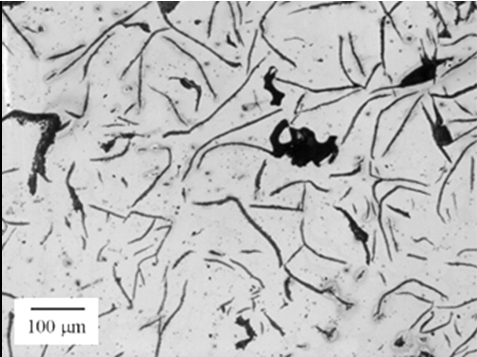
\includegraphics{images/img17.png}
\caption{Ingrandimento al microscopio ottico di un campione di ghisa}
\labfig{img17}
\end{marginfigure}

In un microscopio ottico industriale, tipicamente l’ingrandimento arriva a 1000X. Andando oltre, si ingrandisce semplicemente un’immagine, perdendo in definizione.
Per le ghise, bastano anche 100 ingrandimenti e non è necessario inglobare il campione.

A questo punto di procede con l’operazione di attacco, chimico od elettrochimico.\\
Si immerge il campione in un debole reattivo: in ambito industriale si utilizza il \textbf{NITAL}\index{NITAL}, una soluzione di acido nitrico con tenore dell’1\% in alcol etilico al 5\%, per un tempo limitato di 10-20-60 secondi. Esso deve essere poco reattivo, cioè debolmente aggressivo, perché deve reagire selettivamente: la corrosione avviene per prime le zone a maggior reattività, che sono quelle a maggior energia.

Le zone più reattive sono innanzitutto i bordi di grano: dopo l’attacco si vedranno i bordi di grano e quindi, la struttura del materiale, come nel caso degli acciai ferritici. Si possono studiare, quindi, la dimensione e la tipologia dei grani e la presenza o meno di cementite.

Nel caso di perlite, che è una miscela bi-fasica formata da ferrite e cementite, si vede una zona corrosa a causa della nascita di una pila di corrosione, cioè un anodo e un catodo dovuta alla presenza di due fasi. In questo caso si vedranno zone bianche di ferrite con bordo nero corroso e zone scure di perlite nera, a forma di lamelle corrose.

L’analisi microscopica con microscopio ottico permette di studiare la struttura morfologica e le fasi presenti in un determinato materiale metallico: permette un’analisi quantitativa e qualitativa del materiale.

\begin{marginfigure}[-8cm]
   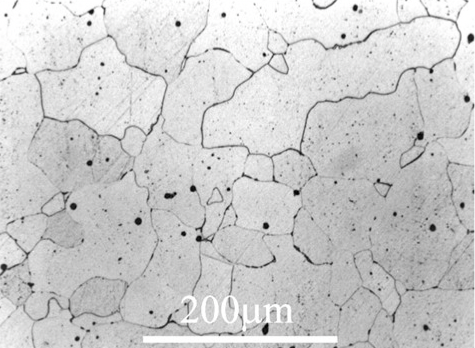
\includegraphics{images/img18.png}
   \caption{Visualizzazione dei bordi di grano in seguito ad un attacco chimico.}
   \labfig{img18}
\end{marginfigure}
   \begin{marginfigure}[-3cm]
   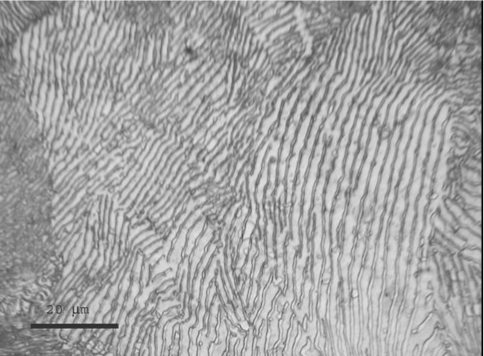
\includegraphics{images/img19.png}
   \caption{Perlite al microscopio ottico}
   \labfig{img18}
   \end{marginfigure}

\section{Microscopio elettronico}\index{microscopio elettronico}

Il principio di funzionamento del microscopio elettronico è basato sull’utilizzo di un fascio di elettroni. In questo caso, il campione non necessita di una superficie riflettente e piana, ma deve essere preparato attraverso una \textbf{perfetta pulizia}, in quanto viene messo sottovuoto. Se il campione fosse sporco, le impurità inquinerebbero il tubo dove vengono emessi gli elettroni.
Il campione viene posto in una soluzione e sottoposto ad ultrasuoni che, vibrando, puliscono il campione.\\
Inoltre, esso deve essere \textbf{conduttivo}, attraverso la metallizzazione con pellicola di oro o di grafite, o l’utilizzo di un ponticello elettronico in rame.

A questo punto il materiale da analizzare viene posto in un tubo, detto \textbf{cannone}, composto da due camere, in una delle quali viene fatto il vuoto. Il filamento presente all’interno del tubo si scalda emettendo un fascio di elettroni che investono il campione: essi vengono riflessi e raccolti per mostrare la topografia del campione.

Esistono microscopi TEM\index{microscopio TEM} (\textbf{Transmission Eletronic Microscope}), utilizzati per ricerche scientifiche dove il campione deve essere così sottile da essere attraversato dagli elettroni. Se non si riesce a renderlo sottile a sufficienza, si utilizza la replica, cioè si copia la superficie su un altro materiale attraverso una pellicola. Tali microscopio raggiungono ingrandimenti da 100000X in su e sono utilizzati per ricerche fini e costose.\\
Vi sono, poi, i microscopi SEM\index{microscopio SEM} (\textbf{Scanning Eletronic Microscope}), chiamato così perché gli elettroni passano per strati mandando l’immagine a video, cioè il campione viene scansionato.

Il microscopio ottico permette di visualizzare un campo 2D, a causa della spianatura della superficie.

Il microscopio elettronico ha il grande vantaggio di dare come risultato immagini tridimensionali, dunque non c’è bisogno della superficie perfettamente piana. Avendo a disposizione la profondità di campo, tale microscopio viene utilizzato nello studio delle superfici di frattura e nello studio della fatica.\\
Infatti, nel caso di una frattura, per utilizzare il microscopio ottico, bisognerebbe spianare la superficie, perdendo le informazioni necessarie all’analisi.

I microscopi elettronici sono dotati di \textbf{microsonde}, che permettono un’analisi chimica
puntuale del materiale: se gli elettroni collidono con il materiale, esso fungerà da anticatodo e quindi da sorgente di raggi X. Ciò permette lo studio della composizione chimica del materiale attraverso un’analisi di fluorescenza: infatti, il reticolo è noto, cioè sono note le costanti reticolari, e con la legge di Bragg si può ricavare la lunghezza d’onda della radiazione emesse e di conseguenza l’energia.

Grazie a questa proprietà i microscopi elettronici sono utili per una topografia 3D della superficie e ancora di più per effettuare analisi chimiche.